%% 11/23/2015
%%%%%%%%%%%%%%%%%%%%%%%%%%%%%%%%%%%%%%%%%%%%%%%%%%%%%%%%%%%%%%%%%%%%%%%%%%%%
% AGUJournalTemplate.tex: this template file is for articles formatted with LaTeX
%
% This file includes commands and instructions
% given in the order necessary to produce a final output that will
% satisfy AGU requirements. 
%
% You may copy this file and give it your
% article name, and enter your text.
%
%%%%%%%%%%%%%%%%%%%%%%%%%%%%%%%%%%%%%%%%%%%%%%%%%%%%%%%%%%%%%%%%%%%%%%%%%%%%
% PLEASE DO NOT USE YOUR OWN MACROS
% DO NOT USE \newcommand, \renewcommand, or \def, etc.
%
% FOR FIGURES, DO NOT USE \psfrag or \subfigure.
% DO NOT USE \psfrag or \subfigure commands.
%%%%%%%%%%%%%%%%%%%%%%%%%%%%%%%%%%%%%%%%%%%%%%%%%%%%%%%%%%%%%%%%%%%%%%%%%%%%
%
% All questions should be e-mailed to latex@agu.org.
%
%%%%%%%%%%%%%%%%%%%%%%%%%%%%%%%%%%%%%%%%%%%%%%%%%%%%%%%%%%%%%%%%%%%%%%%%%%%%
%
% Step 1: Set the \documentclass
%
% There are two options for article format:
%
% 1) PLEASE USE THE DRAFT OPTION TO SUBMIT YOUR PAPERS.
% The draft option produces double spaced output.
% 
% 2) numberline will give you line numbers.

%% To submit your paper:
\documentclass[draft,linenumbers]{AGUJournal}
\draftfalse

%% For final version.
% \documentclass{AGUJournal}

\journalname{Geophysical Research Letters}

\usepackage{gensymb} % To write degrees symbol as \degree
\usepackage{chemformula} % use \ch to write chemical formulas with automatic subscripting

% GRL limit is 12 publication units. Each pub unit is equal to either 500 words, one figure, or one table.  By "words", AGU is only counting the abstract, main article, and captions, not the title, authors, acknowledgements, affiliations, or references. Tables and figures are limited to one full page in the article.

\begin{document}

%% ------------------------------------------------------------------------ %%
%  Title
% 
% (A title should be specific, informative, and brief. Use
% abbreviations only if they are defined in the abstract. Titles that
% start with general keywords then specific terms are optimized in
% searches)
%
%% ------------------------------------------------------------------------ %%

\title{Unexpected decreasing trend in formaldehyde detected from 20-year record at Wollongong, Southeast Australia}

%% ------------------------------------------------------------------------ %%
%
%  AUTHORS AND AFFILIATIONS
%
%% ------------------------------------------------------------------------ %%

% Authors are individuals who have significantly contributed to the
% research and preparation of the article. Group authors are allowed, if
% each author in the group is separately identified in an appendix.)

% List authors by first name or initial followed by last name and
% separated by commas. Use \affil{} to number affiliations, and
% \thanks{} for author notes.  
% Additional author notes should be indicated with \thanks{} (for
% example, for current addresses). 

% Example: \authors{A. B. Author\affil{1}\thanks{Current address, Antartica}, B. C. Author\affil{2,3}, and D. E.
% Author\affil{3,4}\thanks{Also funded by Monsanto.}}

\authors{Kaitlyn J. Lieschke\affil{1}\thanks{Current address, Department of Chemistry, University of California at Berkeley, Berkeley, CA, USA}, Jenny A. Fisher\affil{1,2}, Clare Paton-Walsh\affil{1}, Nicholas B. Jones\affil{1}, Jesse W. Greenslade\affil{1}, Sandy Burden\affil{3}, David W. T. Griffith\affil{1}}

\affiliation{1}{Centre for Atmospheric Chemistry, School of Chemistry, University of Wollongong, Wollongong, NSW, Australia}
\affiliation{2}{School of Earth and Environmental Sciences, University of Wollongong, Wollongong, NSW, Australia}
\affiliation{3}{National Institute for Applied Statistics Research Australia, School of Mathematics and Applied Statistics, University of Wollongong, Wollongong, NSW, Australia}

\correspondingauthor{Kaitlyn Lieschke}{kaitlyn\_lieschke@berkeley.edu}

%% Keypoints, final entry on title page.

% Example: 
% \begin{keypoints}
% \item	List up to three key points (at least one is required)
% \item	Key Points summarize the main points and conclusions of the article
% \item	Each must be 100 characters or less with no special characters or punctuation 
% \end{keypoints}

%  List up to three key points (at least one is required)
%  Key Points summarize the main points and conclusions of the article
%  Each must be 100 characters or less with no special characters or punctuation 

\begin{keypoints}
\item Significant decrease in HCHO observed at Wollongong superimposed on a regional \ch{CH4}-driven increase
\item Lack of trend in November only linked to rising temperature and earlier onset of biogenic emissions
\item Decrease partially attributed to changes in biomass burning but otherwise remains unexplained
\end{keypoints}

%% ------------------------------------------------------------------------ %%
%
%  ABSTRACT
%
% A good abstract will begin with a short description of the problem
% being addressed, briefly describe the new data or analyses, then
% briefly states the main conclusion(s) and how they are supported and
% uncertainties. 
%% ------------------------------------------------------------------------ %%

%% \begin{abstract} starts the second page 

\begin{abstract}
%(limit 150 words)
The response of atmospheric composition to ongoing environmental change remains poorly constrained across much of the southern hemisphere. We use a 20-year record of ground-based total column measurements from Wollongong, southeast Australia to identify a statistically significant decreasing trend in formaldehyde (HCHO) of -1.5 [-2.3, -0.9]\% yr$^{-1}$. The trend is consistently negative across all months except November. Satellite data indicate that the trend at Wollongong is distinctly local and is superimposed on a regional-scale increase driven by changes in methane. In austral summer, coincident decreases in hydrogen cyanide suggest that changes in local biomass burning affect HCHO abundance. However, we find the decreasing trend cannot be fully explained by changes in emissions of HCHO or its precursors, and the overall decrease remains unexplained. In November, an observed increasing temperature trend is consistent with an earlier onset of biogenic emissions in the region, driving increased biogenic HCHO that counteracts the overall decrease.

\end{abstract}


%% ------------------------------------------------------------------------ %%
%
%  TEXT
%
%% ------------------------------------------------------------------------ %%

%%% Suggested section heads:
% \section{Introduction}
% 
% The main text should start with an introduction. Except for short
% manuscripts (such as comments and replies), the text should be divided
% into sections, each with its own heading. 

% Headings should be sentence fragments and do not begin with a
% lowercase letter or number. Examples of good headings are:

% \section{Materials and Methods}
% Here is text on Materials and Methods.
%
% \subsection{A descriptive heading about methods}
% More about Methods.
% 
% \section{Data} (Or section title might be a descriptive heading about data)
% 
% \section{Results} (Or section title might be a descriptive heading about the
% results)
% 
% \section{Conclusions}

% \section{Introduction}
% \section{Materials and Methods}
% \subsection{A descriptive heading about methods}
% \section{Data} (Or section title might be a descriptive heading about data)
% \section{Results} (Or section title might be a descriptive heading about the results)
% \section{Conclusions}

\section{Introduction}

Formaldehyde (\ch{HCHO}) is a short-lived tropospheric pollutant and high-yield oxidation product of non-methane volatile organic compounds (NMVOCs) \citep{Pfister2008,Millet2008a,Franco2016}. Observed HCHO measured from ground-based and satellite remote sensing platforms is frequently used to infer the fluxes of NMVOCS, and in particular isoprene, and can provide insight into how these fluxes are responding to ongoing environmental change \citep{Abbot2003,Millet2008a,Barkley2009,Marais2012,Zhu2014}. Southeast Australia is a global hotspot for both HCHO and isoprene \citep{Pfister2008,Guenther1995,Stavrakou2009,Marais2012}, and is also experiencing rapid and extreme changes in climate \citep{Hughes2003,Murphy2008,IPCC2013B} that could have a significant impact on isoprene emission, HCHO production, and subsequent atmospheric chemistry. Here, we use a long-term record of HCHO from a ground-based remote-sensing instrument at Wollongong, New South Wales, Australia to quantify recent trends in HCHO and investigate their likely drivers.

On a global scale, the main source of atmospheric HCHO is the oxidation of methane (\ch{CH4}) by the hydroxyl radical (\ch{^.OH}) (45-60\%), followed by the oxidation of NMVOCs (20-30\%) \citep{Pfister2008,Dufour2009,Stavrakou2009a,Franco2016}. Direct emissions from fuel combustion, biomass burning and vegetation account for only a minor part of the global HCHO budget, but can be important local sources, particularly during fire events \citep{Holzinger1999,Pfister2008,Dufour2009,Jones2009,Stavrakou2009,Stavrakou2009a,Fortems2012,Franco2016}. HCHO has a short lifetime of only a few hours against photolysis and reaction with \ch{^.OH}  \citep{Fortems2012,Zeng2015}. This makes it an effective indicator of local sources (both primary and secondary) \citep{Jones2009,Palmer2001,Marais2012}. Over Australia, models and satellite data suggest that 40-80\% of HCHO is produced from the oxidation of biogenic NMVOCs, with maximum contributions in the southeast part of the country (New South Wales) where eucalypt-dominated ecosystems are prevalent \citep{Pfister2008,Franco2016,Dufour2009}. However, these regional estimates have not been verified with observations of either isoprene or HCHO.

Recent changes in temperature, global \ch{CH4} abundance and possibly primary HCHO emissions are likely driving changes in HCHO abundance, but the magnitude and effects of these changes in southeast Australia are unknown. Between 1910 and 2010 temperatures in Australia increased 0.8\degree C \citep{ABS2012}, and both biogenic emissions and oxidative chemistry would be sensitive to this change. Globally, methane abundance increased from 1984-1999, stayed almost steady from 1999-2006 and then resumed growing from 2007 onwards \citep{Nisbet2014} with implications for HCHO production \citep{Franco2016}. Decreasing CO emissions over Australia from 2002-2011 have been attributed to changing biomass burning emissions \citet{Yin2015} and declining industrial emissions have been shown to affect other nearby sites \citep{Zeng2012}, both of which could lead to decreases in formaldehyde.

A long-term record of HCHO abundance available from a ground-based Fourier Transform Infrared Spectrometer (FTIR) located at Wollongong, New South Wales (Figure \ref{fig:map}) can provide insight into the implications of these environmental trends.. While short periods of this dataset have been used to evaluate models \citep{Zeng2015}, the full 20-year dataset has not previously been leveraged for understanding atmospheric change in a biogenic-dominated region. This record provides a unique platform to probe changes in a global biogenic hotspot.

Here we evaluate variability and trends in HCHO in southeast Australia, using Wollongong FTIR measurements collected between May 1996 and December 2015. Section 2 describes the measurements and identifies a statistically significant decreasing trend over the 20-year observational period. In Section 3, we use a suite of ground-based and satellite observations of HCHO and related parameters to investigate the drivers of the decreasing HCHO trend. Finally, conclusions are presented in Section 4.

\section{HCHO observations and trend detection}

HCHO measurements were collected from the Fourier Transform Infrared Spectrometer (FTIR) at the Wollongong site of the Network for the Detection of Atmospheric Composition Change (NDACC), located at the University of Wollongong (34.45\degree S, 150.88\degree E, 30 m above sea level, see Figure \ref{fig:map}). Measurements are derived from ground-based solar infrared absorption spectra \citep{Griffith1998,Te2016}. Figure \ref{fig:hcho_ts}a shows the individual retrievals of HCHO total column abundance from May 1996 to December 2015. The influence of local fire events can be seen particularly in December 2001 - January 2002, January 2003 and October 2013 \citep{Paton-Walsh2004,Paton-Walsh2005,Paton-Walsh2010,Rea2016}. The mean seasonal cycle, shown in Figure \ref{fig:hcho_ts}b, shows that HCHO peaks in austral summer due the large influence from biogenic NMVOC emissions at this time of year \citep{Jones2009,Zeng2012}.

\begin{figure}[h!]
  \begin{center}
    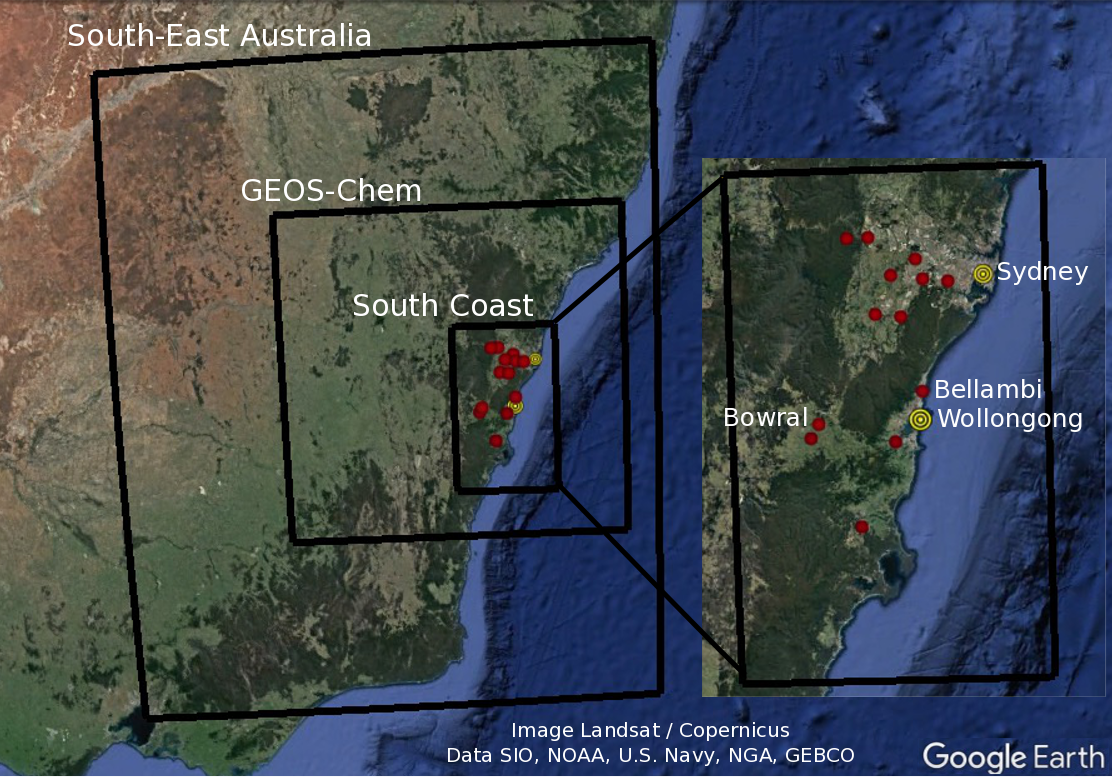
\includegraphics[width=0.7\textwidth]{Wollongong_region_map}
      \caption{Map of southeast Australia showing the location of the FTIR at Wollongong,  Bureau of Meteorology sites (red) and three regions over which satellite data was averaged (black boxes). The city of Sydney is also shown for context.}
  \label{fig:map}
  \end{center}
\end{figure}

\begin{figure}[h!]
  \begin{center}
    \includegraphics[width=0.7\textwidth]{HCHO_OE_timeseries_Wollongong_edited}
      \caption{HCHO observations from FTIR at Wollongong, southeast Australia from May 1996 - December 2015 showing (a) the long term time series, (b) the mean seasonal cycle, with shaded regions representing the 95\% confidence interval of the observations, and (c) the deseasonalised anomalies and trend in HCHO from May 1996 - December 2015 (red solid line) and from February 2003 - September 2013 (black dashed line).}
  \label{fig:hcho_ts}
  \end{center}
\end{figure}

Trends in HCHO abundance were calculated using the Thielsen function in the R package OpenAir \citep{Carslaw2012}. All trends are significant to \textit{p} \textless 0.05 and are reported along with the 95\% confidence interval in brackets. Figure \ref{fig:hcho_ts}c shows the calculated trend in HCHO of -1.5 [-2.3, -0.9]\% yr$^{-1}$, after accounting for seasonality and autocorrelation. To exclude the effects of large fire events, we also calculated the trend from February 2003 to September 2013 (black dashed line in Figure \ref{fig:hcho_ts}c), and found that it doubled in magnitude to -3.0 [-4.3, -2.0]\% yr$^{-1}$.

To elucidate possible causes of the observed HCHO trend, we  calculated the trend in HCHO abundance for each month, as different source and sink influences have different seasonality. HCHO production from biogenic NMVOC sources peaks in austral summer (November-February) \citep{Zeng2015}, while local biomass burning peaks in October-January \citep{Edwards2006,Zeng2015}, and anthropogenic emissions have limited seasonality \citep{Streets2003,Helmig2009}. Methane oxidation is largest in summer due to increased OH production \citep{Khalil1983}, but the impact on HCHO may be offset by more rapid HCHO oxidative loss. While the mean seasonal variation of HCHO at Wollongong (Figure \ref{fig:hcho_ts}b) is driven by the seasonality of biogenic NMVOC emissions, other influences not visible in the multi-year mean could impart a seasonal signature to the trends. Figure \ref{fig:hcho_mon} shows that the monthly trends are strongly negative (between -1 and -2.5 \% yr$^{-1}$) except in November, when there is no significant trend. With the exception of November, the monthly trends are largely consistent with one another and with the overall trend (shown in Figure \ref{fig:hcho_mon} as the dashed red line). 

\begin{figure}[h]
  \begin{center}
    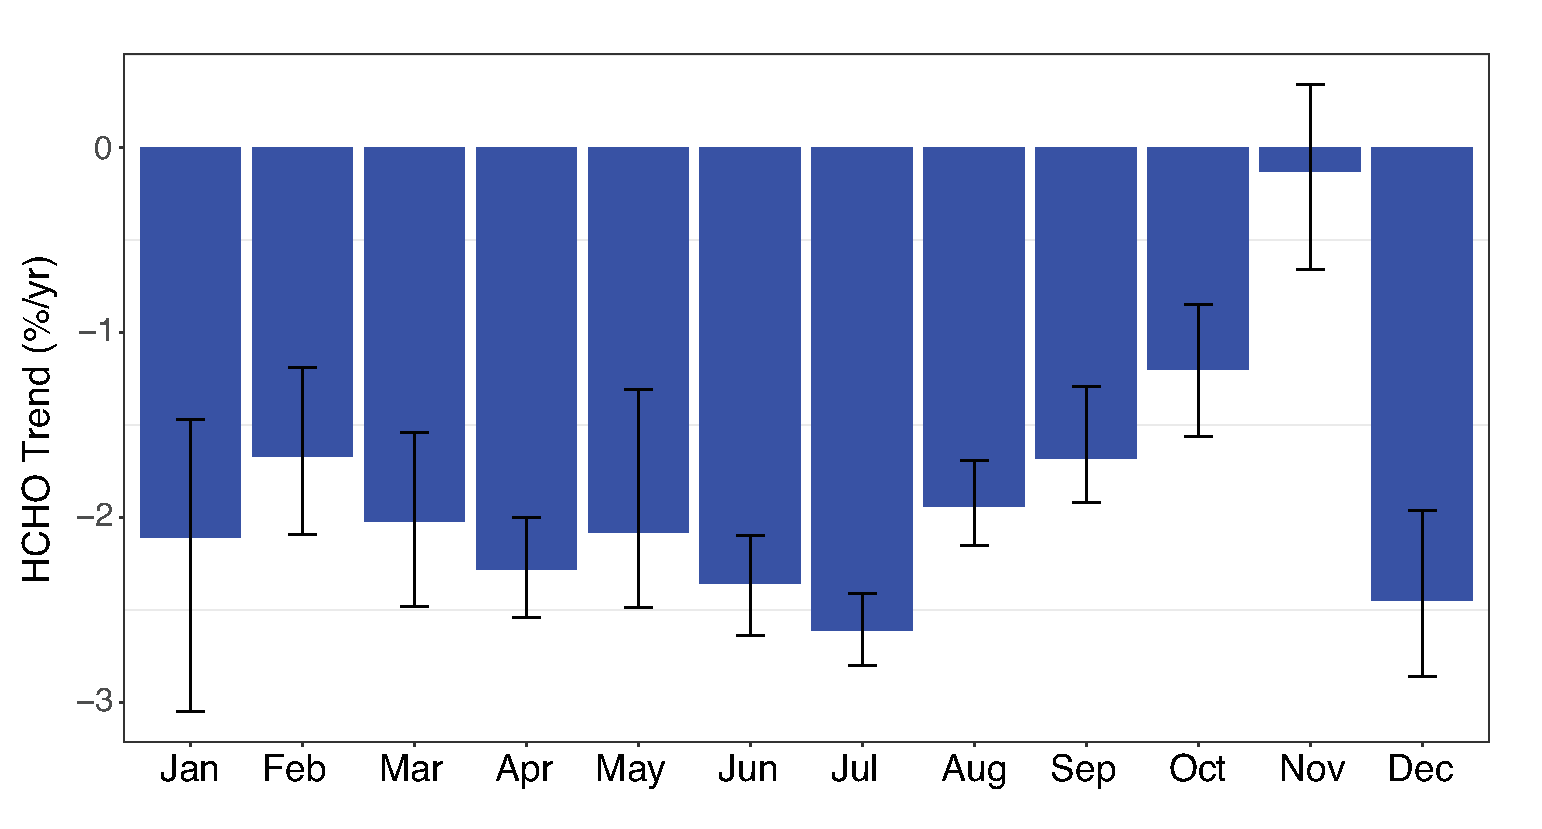
\includegraphics[width=0.65\textwidth]{HCHO_OE_Wollongong_monthly_trends}
      \caption{Monthly trends in HCHO total columns from FTIR observations at Wollongong, southeast Australia from May 1996 - December 2015. The overall trend (calculated from all data) is shown by the red dashed line. Solid lines represent the 95\% confidence interval for each monthly trend.}
  \label{fig:hcho_mon}
  \end{center}
\end{figure}


\section{Diagnosis of observed trends}

\subsection{Biogenic emissions}
In southeast Australia, models suggest oxidation of NMVOCs is the dominant source of HCHO ($\sim$80\% \citep{Pfister2008}). Isoprene accounts for approximately half of the total NMVOC emissions globally \citep{Guenther2012}, including in Australia \citep{Emmerson2016}. Biogenic emissions of isoprene are strongly temperature dependent, with a threshold of around 12\degree C below which no isoprene is emitted \citep{Oku2014}. Above this threshold, isoprene emissions increase substantially up to a thermal optimum of 35 to 40\degree C \citep{Monson1992,Sharkey2001}. This suggests that observed temperature changes in southeast Australia \citep{ABS2012} could be affecting the emission of biogenic HCHO precursors and driving the observed changes in HCHO abundance at Wollongong.

To test this hypothesis, we used temperature observations from sites around Wollongong (see Figure \ref{fig:map}) provided by the Australian Bureau of Meteorology (BoM). Due to the short lifetime of both isoprene (typically less than one hour) \citep{Palmer2003,Crutzen1999} and HCHO (on the order of a few hours) \citep{Palmer2003,DeSmedt2015}, only sites within 100 km of Wollongong were considered close enough to be representative of biogenic emission regions that potentially influence the site. This distance should also be sufficient to account for slower HCHO production via low NOx chemistry during transport of precursor NMVOCs.

We calculated overall and monthly trends for each BoM site using the daily minimum and maximum temperature data for all available dates from 1997-2015. Mean temperature data were not available. Taken together, the sites showed no clear indication of consistent temperature change over the region. Only a small fraction of the sites showed a trend in either the overall or monthly data, and these were not consistent across sites or across months. We also calculated the regional mean temperature trends using the observations from all sites with available data for 1997-2014 (including only days for which temperature data were available from all sites). While no overall trends were seen, an increase of +0.1 [0.0, +0.2] \degree C yr$^{-1}$ was noted in November, equivalent to +0.7\% yr$^{-1}$.

We further investigated the possible role of temperature-driven changes in biogenic emissions using temperature observations from Bowral, an inland site located in a highly vegetated region approximately 45 km west of Wollongong (see Figure \ref{fig:map}) that could be a large source region for HCHO precursors. Temperature measurements at Bowral were only available at 09:00 and 15:00 local standard time from January 1997 to January 2015. As with the multi-site mean, no overall trend was detected. In November, however, the observations showed an increasing trend in temperature of +0.2 [0.0, +0.3] \degree C yr$^{-1}$ in the morning (09:00) and +0.2 [0.0, +0.4] \degree C yr$^{-1}$  in the afternoon (15:00), equivalent to +1\% yr$^{-1}$.

Given the strong sensitivity of isoprene emissions to atmospheric temperature, it is likely that the November warming observed both at Bowral and in the multi-site mean has driven an increase in biogenic emissions in the southeast Australian region. Minimum temperatures in this area typically reach the threshold for isoprene emission (12\degree C \citep{Oku2014}) sometime in November or December, and at Bowral the mean minimum temperature in November rose from below 12\degree C to above 12\degree C over this time period. The warming may be associated with both a higher magnitude and an earlier onset of isoprene emissions in the region in November, with subsequent oxidation leading to an increase in biogenically-derived HCHO. We therefore suggest that the overall strong decreasing trend in HCHO observed during the rest of the year is being offset in November by an increase in biogenic HCHO - with the net effect being no significant change in November HCHO over the past 20 years.

\subsection{Methane oxidation}
On a global scale, \ch{CH4} oxidation is the largest source of HCHO ($\sim$50\% \citep{Pfister2008}). Changes in background \ch{CH4} abundance have been shown to affect HCHO observed at other sites and could be impacting the HCHO observations at Wollongong. At Jungfraujoch, for example, \citet{Franco2016} found changes in HCHO and \ch{CH4} between 1998 and 2015 were strongly correlated. Using FTIR measurements, the authors found a decrease in HCHO abundance of -3.68 +/- 1.00\% yr$^{-1}$ from 1996-2002, the period when global \ch{CH4} levels stabilised \citep{Dlugokencky2003,Aydin2011,Simpson2012}, and an increase in HCHO abundance of +0.81 +/- 0.62\% yr$^{-1}$ from 2003-2015, when \ch{CH4} levels were stable followed by resumed growth \citep{Kirschke2013,Nisbet2014}.

The trends observed at Wollongong do not seem to be similarly affected by background changes in \ch{CH4} oxidation. While the FTIR at Jungfraujoch samples the free troposphere where \ch{CH4} oxidation is the dominant HCHO source, the Wollongong FTIR is just above sea level and is therefore more sensitive to local processes and less sensitive to background processes. In addition, the timing of the observed HCHO trends is not consistent with the timing of changes in global \ch{CH4} abundance. From 2003-2015, when methane levels were stable then increasing \citep{Nisbet2014} and HCHO increased at Jungfraujoch \citep{Franco2016}, Wollongong HCHO observations showed a large decrease of -2.6 [-3.3, -1.8] \% yr$^{-1}$.

We expect that any \ch{CH4}-driven change in HCHO would be at least regional in scale. To further explore the impact of \ch{CH4} oxidation on changing HCHO in southeast Australia, we used satellite observations of HCHO total column measurements from the Ozone Monitoring Instrument (OMI) level 2 global swath product, OMHCHO. For details of the instrument and retrieval, see Section S1 in the Supporting Information. We chose OMI rather than other satellite products as it had the longest continuous overlap with the FTIR record. Satellite measurements were averaged daily and gridded to obtain mean HCHO abundance from 2005-2015 over the three regions shown in Figure \ref{fig:map}. The ``South Coast'' region (33.5-35.5\degree S x 150.0-151.5\degree E) contains land within 100 km of Wollongong and limited ocean cover and was selected to represent the region over which isoprene and/or HCHO could be expected to travel within their lifetimes. The ``GEOS-Chem'' region corresponds to the size of a coarse resolution grid box simulated by the GEOS-Chem CTM (32-36\degree S x 147.5-152.5\degree E, see Section S2 in the Supporting Information). The ``Southeast Australia'' region covers the wider regional area (30-38\degree S x 145-153\degree E).

The decreasing HCHO trend seen in the Wollongong FTIR data is not evident in the OMI data, suggesting it is a local rather than regional phenomenon. OMI measurements over the South Coast region showed no significant trend over the 2005-2015 period. The larger GEOS-Chem and Southeast Australian regions showed increases in HCHO of +0.9 [+0.4, +1.6] \% yr$^{-1}$ and +1.5 [+0.8, +2.0] \% yr$^{-1}$, respectively. These are opposite in sign to the trend calculated from the FTIR measurements which, when limited to the 2005-2015 OMI period, still showed a decrease of -2.5 [-3.8, -1.6]\% yr$^{-1}$ in HCHO. Monthly trends were generally insignificant over this shorter period, except for an August increase in the OMI data for all three regions and January, May, and July-September decreases in the Wollongong FTIR measurements.

The observed regional-scale increase in OMI HCHO during this period can be attributed to changes in global \ch{CH4} abundance, as seen elsewhere \citep{Franco2016}. The decreasing trend at Wollongong, however, is inconsistent with this increasing trend -- suggesting that the greater regional increase in HCHO is being overpowered by local changes at Wollongong that cannot be attributed to \ch{CH4}.

\subsection{Emissions and transport}
Primary emissions of HCHO from biomass burning and anthropogenic sources account for only 0.4-0.8\% of the global budget \citep{Pfister2008,Fortems2012,Zeng2015}. However, these can be important local sources, particularly when large emission events occur \citep{Stavrakou2009}. To investigate the potential impact of these direct emissions on HCHO at Wollongong, we compared the observed  trends in HCHO to those for hydrogen cyanide (HCN) and carbon monoxide (CO), also measured by the Wollongong FTIR. We use HCN as a tracer of biomass burning, its primary source \citep{Li2000,Li2003,Li2009}. CO has major sources from \ch{CH4} and NMVOC oxidation, biomass burning, and anthropogenic emissions \citep{Zeng2015,Fisher2015,Yin2015}. We use it here to provide an indication of changes in anthropogenic emissions, as changes in the other CO sources should also be apparent in either HCN (biomass burning) or HCHO (oxidation).

\begin{figure}[h!]
  \begin{center}
    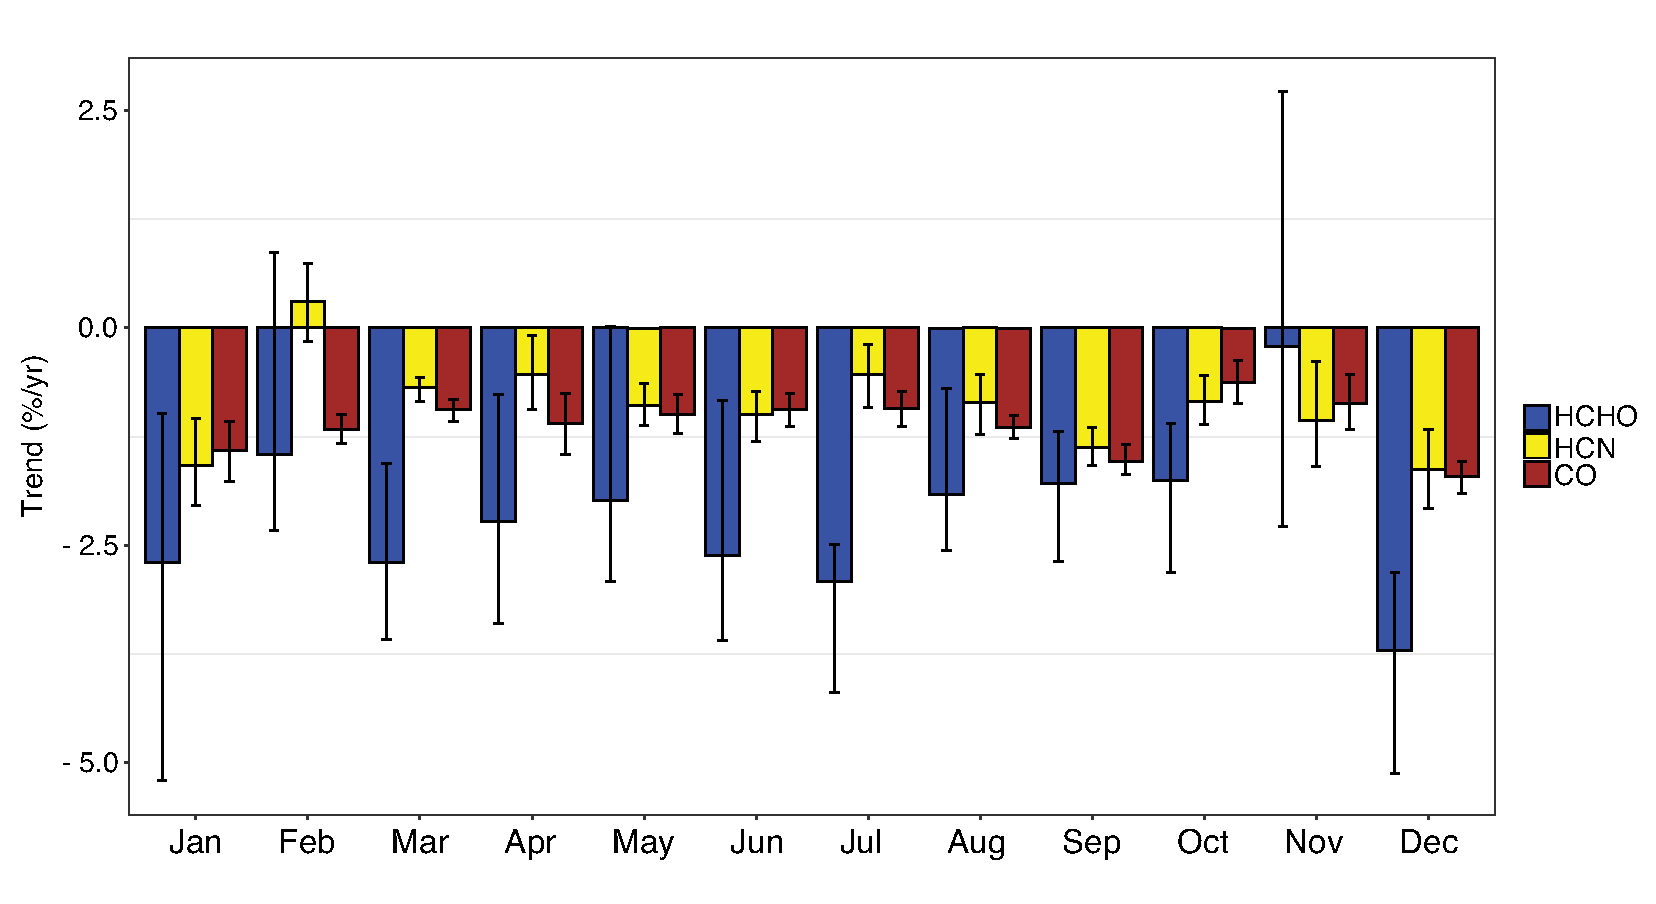
\includegraphics[width=0.8\textwidth]{all_tg_monthly_trends_wollongong}
      \caption{Monthly trends in HCHO (blue), HCN (yellow), and CO (brown) total columns at Wollongong, Australia from May 1997 to April 2014 calculated from FTIR observations, along with associated 95\% confidence interval.}
  \label{fig:alltg_trends}
  \end{center}
\end{figure}

Figure \ref{fig:alltg_trends} compares monthly trends in HCHO, CO and HCN for the period of time over which measurements of all three gases overlapped (May 1997 to April 2014). Over this period, the year-round abundance of all three gases decreased with trends of -1.9 [-2.7, -1.5] \% yr$^{-1}$, -1.0 [-1.5, -0.7] \% yr$^{-1}$ and -0.76 [-1.66, 0.1] \% yr$^{-1}$ for HCHO, CO and HCN, respectively. Figure \ref{fig:alltg_trends} shows that the monthly trends are generally negative for all three species, and HCN and CO trends are nearly always similar in magnitude. For both HCN and CO, the largest negative trends are seen in December-January, when local fires frequently occur \citep{Zeng2015,Paton-Walsh2004,Paton-Walsh2005,Paton-Walsh2010,Rea2016}, and in September, when southern hemisphere biomass burning peaks \citep{Edwards2006}. This suggests that changes in biomass burning frequency and/or intensity are driving a decrease in both species during these months. The large observed decreases in HCHO in December-January could also be attributable at least in part to the same source; however, large decreases in HCHO in austral autumn and winter (March-July) do not appear to be correlated with trends in either HCN or CO. This suggests that the overall negative trend in HCHO at Wollongong cannot be fully explained by changing emissions from  biomass burning and/or anthropogenic sources, although these may contribute in summer.

We also investigated whether a change in meteorology was likely to have caused a change in the transport of HCHO or its precursors from source regions to Wollongong. We calculated trends in both wind speed and direction using BoM measurements from the nearby station at Bellambi (see Figure \ref{fig:map}). Neither variable showed compelling evidence for a change in transport in this region.

Finally, we attempted to diagnose the trends using the GEOS-Chem chemical transport model (see Section S2 in the Supporting Information). To prevent introducing artificial trends from changes in model inputs, we were limited to the 1997-2011 period for which consistent biomass burning emissions were available. We found that observed trends from the FTIR were weaker over this period (see Figure S2 in the Supporting Information). While the model successfully captured the observed seasonal variability, simulated 1997-2011 trends were not consistent with the observations, and so the model could not be used to shed further light on the drivers of the observed trend.

\section{Summary and Conclusion}

We have used a 20-year record of ground-based FTIR measurements from Wollongong (New South Wales, Australia) to identify a significant decreasing trend in HCHO in southeast Australia of -1.5\% yr$^{-1}$ from 1996 to 2015. Monthly trends calculated from the same dataset show that the HCHO trend is consistently negative throughout the year, with the exception of November when no significant trend is detected.

Using a variety of related datasets, we tested several possible explanations for the drivers of the decreasing trend at Wollongong. OMI satellite data suggested that at the larger (regional) scale, HCHO in southeast Australia is increasing rather than decreasing, likely driven by growth in \ch{CH4} (and therefore \ch{CH4} oxidation leading to HCHO production) in the background atmosphere. Comparison to others species available in the FTIR record (HCN, CO) indicated a decrease in the frequency and/or intensity of local fires that could be partially responsible for the observed HCHO changes in December-January. However, changes in local emissions are insufficient to explain the decreasing trend seen throughout the rest of the year, and the overall decrease in HCHO at Wollongong remains unexplained.

Temperature observations from across the region, including at a densely vegetated site west of Wollongong, showed a warming trend over the past 20 years in November only, coincident with the only month during which HCHO did not decrease. At this time of year, the seasonal transition from spring to summer is accompanied by increasing temperature, eventually crossing the threshold required for isoprene emission. We suggest that the observed November warming in the Wollongong region is driving an earlier onset of isoprene emissions -- and with it an increase in HCHO production that is sufficient to offset the otherwise decreasing trend seen during the rest of the year. Projected future warming \citep{Hughes2003,Alexander2009} could further lengthen the season during which biogenic VOCs are emitted in this region, and the associated increase in HCHO production may eventually overwhelm the unexplained HCHO decreases that have occurred to-date.


%Text here ===>>>

%%

%  Numbered lines in equations:
%  To add line numbers to lines in equations,
%  \begin{linenomath*}
%  \begin{equation}
%  \end{equation}
%  \end{linenomath*}



%% Enter Figures and Tables near as possible to where they are first mentioned:
%
% DO NOT USE \psfrag or \subfigure commands.
%
% Figure captions go below the figure.
% Table titles go above tables;  other caption information
%  should be placed in last line of the table, using
% \multicolumn2l{$^a$ This is a table note.}
%
%----------------
% EXAMPLE FIGURE
%
% \begin{figure}[h]
% \centering
% when using pdflatex, use pdf file:
% \includegraphics[width=20pc]{figsamp.pdf}
%
% when using dvips, use .eps file:
% \includegraphics[width=20pc]{figsamp.eps}
%
% \caption{Short caption}
% \label{figone}
%  \end{figure}
%
% ---------------
% EXAMPLE TABLE
%
% \begin{table}
% \caption{Time of the Transition Between Phase 1 and Phase 2$^{a}$}
% \centering
% \begin{tabular}{l c}
% \hline
%  Run  & Time (min)  \\
% \hline
%   $l1$  & 260   \\
%   $l2$  & 300   \\
%   $l3$  & 340   \\
%   $h1$  & 270   \\
%   $h2$  & 250   \\
%   $h3$  & 380   \\
%   $r1$  & 370   \\
%   $r2$  & 390   \\
% \hline
% \multicolumn{2}{l}{$^{a}$Footnote text here.}
% \end{tabular}
% \end{table}

%% SIDEWAYS FIGURE and TABLE 
% AGU prefers the use of {sidewaystable} over {landscapetable} as it causes fewer problems.
%
% \begin{sidewaysfigure}
% \includegraphics[width=20pc]{figsamp}
% \caption{caption here}
% \label{newfig}
% \end{sidewaysfigure}
% 
%  \begin{sidewaystable}
%  \caption{Caption here}
% \label{tab:signif_gap_clos}
%  \begin{tabular}{ccc}
% one&two&three\\
% four&five&six
%  \end{tabular}
%  \end{sidewaystable}

%% If using numbered lines, please surround equations with \begin{linenomath*}...\end{linenomath*}
%\begin{linenomath*}
%\begin{equation}
%y|{f} \sim g(m, \sigma),
%\end{equation}
%\end{linenomath*}

%%% End of body of article

%%%%%%%%%%%%%%%%%%%%%%%%%%%%%%%%
%% Optional Appendix goes here
%
% The \appendix command resets counters and redefines section heads
%
% After typing \appendix
%
%\section{Here Is Appendix Title}
% will show
% A: Here Is Appendix Title
%
%\appendix
%\section{Here is a sample appendix}

%%%%%%%%%%%%%%%%%%%%%%%%%%%%%%%%%%%%%%%%%%%%%%%%%%%%%%%%%%%%%%%%
%
% Optional Glossary, Notation or Acronym section goes here:
%
%%%%%%%%%%%%%%  
% Glossary is only allowed in Reviews of Geophysics
%  \begin{glossary}
%  \term{Term}
%   Term Definition here
%  \term{Term}
%   Term Definition here
%  \term{Term}
%   Term Definition here
%  \end{glossary}

%
%%%%%%%%%%%%%%
% Acronyms
%   \begin{acronyms}
%   \acro{Acronym}
%   Definition here
%   \acro{EMOS}
%   Ensemble model output statistics 
%   \acro{ECMWF}
%   Centre for Medium-Range Weather Forecasts
%   \end{acronyms}

%
%%%%%%%%%%%%%%
% Notation 
%   \begin{notation}
%   \notation{$a+b$} Notation Definition here
%   \notation{$e=mc^2$} 
%   Equation in German-born physicist Albert Einstein's theory of special
%  relativity that showed that the increased relativistic mass ($m$) of a
%  body comes from the energy of motion of the body—that is, its kinetic
%  energy ($E$)—divided by the speed of light squared ($c^2$).
%   \end{notation}




%%%%%%%%%%%%%%%%%%%%%%%%%%%%%%%%%%%%%%%%%%%%%%%%%%%%%%%%%%%%%%%%
%
%  ACKNOWLEDGMENTS
%
% The acknowledgments must list:
%
% •	All funding sources related to this work from all authors
%
% •	Any real or perceived financial conflicts of interests for any
%	author
%
% •	Other affiliations for any author that may be perceived as
% 	having a conflict of interest with respect to the results of this
% 	paper.
%
% •	A statement that indicates to the reader where the data
% 	supporting the conclusions can be obtained (for example, in the
% 	references, tables, supporting information, and other databases).
%
% It is also the appropriate place to thank colleagues and other contributors. 
% AGU does not normally allow dedications.


\acknowledgments
We wish to acknowledge Voltaire Velazco and the entire UOW FTIR team for their contribution to the NDACC data over the years. The standard NDACC data for Wollongong are available at ftp.cpc.ncep.noaa.gov/ndacc/station/wollong. The specific version used here are available by contacting the authors. This work was funded by the University of Wollongong through the Faculty of Science, Medicine and Health and a Vice Chancellor's Postdoctoral Fellowship to J. A. Fisher. The remote sensing program at the University of Wollongong has been supported by the Australian Research Council (ARC) through a series of grants, the most recent grant being DP160101598. This research was undertaken with the assistance of resources provided at the NCI National Facility systems at the Australian National University through the National Computational Merit Allocation Scheme supported by the Australian Government.


%% ------------------------------------------------------------------------ %%
%% Citations

% Please use ONLY \citet and \citep for reference citations.
% DO NOT use other cite commands (e.g., \cite, \citeyear, \nocite, \citealp, etc.).


%% Example \citet and \citep:
%  ...as shown by \citet{Boug10}, \citet{Buiz07}, \citet{Fra10},
%  \citet{Ghel00}, and \citet{Leit74}. 

%  ...as shown by \citep{Boug10}, \citep{Buiz07}, \citep{Fra10},
%  \citep{Ghel00, Leit74}. 

%  ...has been shown \citep [e.g.,][]{Boug10,Buiz07,Fra10}.



%%  REFERENCE LIST AND TEXT CITATIONS
%
% Either type in your references using
%
% \begin{thebibliography}{}
% \bibitem[{\textit{Kobayashi et~al.}}(2003)]{R2013} Kobayashi, T.,
% Tran, A.~H., Nishijo, H., Ono, T., and Matsumoto, G.  (2003).
% Contribution of hippocampal place cell activity to learning and
% formation of goal-directed navigation in rats. \textit{Neuroscience}
% 117, 1025--1035.
%
% \bibitem{}
% Text
% \end{thebibliography}
%
%%%%%%%%%%%%%%%%%%%%%%%%%%%%%%%%%%%%%%%%%%%%%%%
% Or, to use BibTeX:
%
% Follow these steps
%
% 1. Type in \bibliography{<name of your .bib file>} 
%\bibliography{formaldehydetrends}
%    Run LaTeX on your LaTeX file.
%
% 2. Run BiBTeX on your LaTeX file.
%
% 3. Open the new .bbl file containing the reference list and
%   copy all the contents into your LaTeX file here.
%
% 4. Run LaTeX on your new file which will produce the citations.
%
% AGU does not want a .bib or a .bbl file. Please copy in the contents of your .bbl file here.

%% After you run BibTeX, Copy in the contents of the .bbl file here:
\begin{thebibliography}{51}
\providecommand{\natexlab}[1]{#1}
\expandafter\ifx\csname urlstyle\endcsname\relax
  \providecommand{\doi}[1]{doi:\discretionary{}{}{}#1}\else
  \providecommand{\doi}{doi:\discretionary{}{}{}\begingroup
  \urlstyle{rm}\Url}\fi

\bibitem[{\textit{Abbot et~al.}(2003)\textit{Abbot, Palmer, Martin, Chance,
  Jacob, and Guenther}}]{Abbot2003}
Abbot, D.~S., P.~I. Palmer, R.~V. Martin, K.~V. Chance, D.~J. Jacob, and
  A.~Guenther (2003), {Seasonal and interannual variability of North American
  isoprene emissions as determined by formaldehyde column measurements from
  space}, \textit{Geophysical Research Letters}, \textit{30}(17),
  \doi{10.1029/2003GL017336}.

\bibitem[{\textit{ABS}(2012)}]{ABS2012}
ABS, Australian Bureau of Statistics (2012), {Geography and Climate: Australia's Climate}, in
  \textit{2012 Year Book Australia}, chap.~1, pp. 75--92, Canberra.

\bibitem[{\textit{Alexander and Arblaster}(2009)}]{Alexander2009}
Alexander, L.~V., and J.~M. Arblaster (2009), {Assessing trends in observed and
  modelled climate extremes over Australia in relation to future projections},
  \textit{International Journal of Climatology}, \textit{29}, 417--435,
  \doi{10.1002/joc.1730}.

\bibitem[{\textit{Aydin et~al.}(2011)\textit{Aydin, Verhulst, Saltzman, Battle,
  Montzka, Blake, Tang, and Prather}}]{Aydin2011}
Aydin, M., K.~R. Verhulst, E.~S. Saltzman, M.~O. Battle, S.~A. Montzka, D.~R.
  Blake, Q.~Tang, and M.~J. Prather (2011), {Recent decreases in fossil-fuel
  emissions of ethane and methane derived from firn air}, \textit{Nature},
  \textit{476}, 198--201, \doi{10.1038/nature10352}.

\bibitem[{\textit{Barkley et~al.}(2009)\textit{Barkley, Palmer, {De Smedt},
  Karl, Guenther, and {Van Roozendael}}}]{Barkley2009}
Barkley, M.~P., P.~I. Palmer, I.~{De Smedt}, T.~Karl, A.~Guenther, and M.~{Van
  Roozendael} (2009), {Regulated large-scale annual shutdown of Amazonian
  isoprene emissions?}, \textit{Geophysical Research Letters}, \textit{36},
  \doi{10.1029/2008GL036843}.

\bibitem[{\textit{Bindoff et~al.}(2013)\textit{Bindoff, Stott, AchutaRao,
  Allen, Gillett, Gutzler, Hansingo, Hegerl, Hu, Jain, Mokhov, Overland,
  Perlwitz, Sebbari, and Zhang}}]{IPCC2013B}
Bindoff, N.~L., P.~A. Stott, K.~M. AchutaRao, M.~R. Allen, N.~Gillett,
  D.~Gutzler, K.~Hansingo, G.~Hegerl, Y.~Hu, S.~Jain, I.~I. Mokhov,
  J.~Overland, J.~Perlwitz, R.~Sebbari, and X.~Zhang (2013), {Detection and
  Attribution of Climate Change: from Global to Regional}, in \textit{Climate
  Change 2013: The Physical Science Basis. Contribution of Working Group I to
  the Fifth Assessment Report of the Intergovernmental Panel on Climate Change
  [Stocker, T.F., D. Qin, G.-K. Plattner, M. Tignor, S.K. Allen, J. Boschung,
  A. Nauels, Y. Xia, V. Bex and P.M. Midgley (eds)]}, pp. 1217-1308, Cambridge University Press, Cambridge,
  United Kingdom and New York, NY, USA, \doi{10.1017/CBO9781107415324.028}.

\bibitem[{\textit{Carslaw and Ropkins}(2012)}]{Carslaw2012}
Carslaw, D.~C., and K.~Ropkins (2012), {openair - An R package for air quality
  data analysis}, \textit{Environmental Modelling and Software},
  \textit{27-28}, 52--61, \doi{10.1016/j.envsoft.2011.09.008}.

\bibitem[{\textit{Crutzen et~al.}(1999)\textit{Crutzen, Lawrence, and
  P{\"{o}}schl}}]{Crutzen1999}
Crutzen, P.~J., M.~G. Lawrence, and U.~P{\"{o}}schl (1999), {On the background
  photochemistry of tropospheric ozone}, \textit{Tellus}, \textit{51A-B},
  123--146, \doi{10.1034/j.1600-0870.1999.t01-1-00010.x}.

\bibitem[{\textit{{De Smedt} et~al.}(2015)\textit{{De Smedt}, Stavrakou,
  Hendrick, Danckaert, Vlemmix, Pinardi, Theys, Lerot, Gielen, Vigouroux,
  Hermans, Fayt, Veefkind, M{\"{u}}ller, and {Van Roozendael}}}]{DeSmedt2015}
{De Smedt}, I., T.~Stavrakou, F.~Hendrick, T.~Danckaert, T.~Vlemmix,
  G.~Pinardi, N.~Theys, C.~Lerot, C.~Gielen, C.~Vigouroux, C.~Hermans, C.~Fayt,
  P.~Veefkind, J.~F. M{\"{u}}ller, and M.~{Van Roozendael} (2015), {Diurnal,
  seasonal and long-term variations of global formaldehyde columns inferred
  from combined OMI and GOME-2 observations}, \textit{Atmospheric Chemistry and
  Physics}, \textit{15}, 12,519--12,545, \doi{10.5194/acp-15-12519-2015}.

\bibitem[{\textit{Dlugokencky et~al.}(2003)\textit{Dlugokencky, Houweling,
  Bruhwiler, Masarie, Lang, Miller, and Tans}}]{Dlugokencky2003}
Dlugokencky, E.~J., S.~Houweling, L.~Bruhwiler, K.~A. Masarie, P.~M. Lang,
  J.~B. Miller, and P.~P. Tans (2003), {Atmospheric methane levels off:
  Temporary pause or a new steady-state?}, \textit{Geophysical Research
  Letters}, \textit{30}, \doi{10.1029/2003GL018126}.

\bibitem[{\textit{Dufour et~al.}(2009)\textit{Dufour, Szopa, Barkley, Boone,
  Perrin, Palmer, and Bernath}}]{Dufour2009}
Dufour, G., S.~Szopa, M.~P. Barkley, C.~D. Boone, A.~Perrin, P.~I. Palmer, and
  P.~F. Bernath (2009), {Global upper-tropospheric formaldehyde: seasonal
  cycles observed by the ACE-FTS satellite instrument}, \textit{Atmospheric
  Chemistry and Physics}, \textit{9}, 3893--3910,
  \doi{10.5194/acpd-9-1051-2009}.

\bibitem[{\textit{Edwards et~al.}(2006)\textit{Edwards, Emmons, Gille, Chu,
  Atti{\'{e}}, Giglio, Wood, Haywood, Deeter, Massie, Ziskin, and
  Drummond}}]{Edwards2006}
Edwards, D.~P., L.~K. Emmons, J.~C. Gille, A.~Chu, J.-L. Atti{\'{e}},
  L.~Giglio, S.~W. Wood, J.~Haywood, M.~N. Deeter, S.~T. Massie, D.~C. Ziskin,
  and J.~R. Drummond (2006), {Satellite-observed pollution from Southern
  Hemisphere biomass burning}, \textit{Journal of Geophysical Research},
  \textit{111}, \doi{10.1029/2005JD006655}.

\bibitem[{\textit{Emmerson et~al.}(2016)\textit{Emmerson, Galbally, Guenther,
  Paton-Walsh, Guerette, Cope, Keywood, Lawson, Molloy, Dunne, Thatcher, Karl,
  and Maleknia}}]{Emmerson2016}
Emmerson, K.~M., I.~E. Galbally, A.~B. Guenther, C.~Paton-Walsh, E.-A.
  Guerette, M.~E. Cope, M.~D. Keywood, S.~J. Lawson, S.~B. Molloy, E.~Dunne,
  M.~Thatcher, T.~Karl, and S.~D. Maleknia (2016), {Current estimates of
  biogenic emissions from eucalypts uncertain for southeast Australia},
  \textit{Atmospheric Chemistry and Physics}, \textit{16}, 6997--7011,
  \doi{10.5194/acp-16-6997-2016}.

\bibitem[{\textit{Fisher et~al.}(2015)\textit{Fisher, Wilson, Zeng, Williams,
  Emmons, Langenfelds, Krummel, and Steele}}]{Fisher2015}
Fisher, J.~A., S.~R. Wilson, G.~Zeng, J.~E. Williams, L.~K. Emmons, R.~L.
  Langenfelds, P.~B. Krummel, and L.~P. Steele (2015), {Seasonal changes in the
  tropospheric carbon monoxide profile over the remote Southern Hemisphere
  evaluated using multi-model simulations and aircraft observations},
  \textit{Atmospheric Chemistry and Physics}, \textit{15}, 3217--3239,
  \doi{10.5194/acp-15-3217-2015}.

\bibitem[{\textit{Fortems-Cheiney et~al.}(2012)\textit{Fortems-Cheiney,
  Chevallier, Pison, Bousquet, Saunois, Szopa, Cressot, Kurosu, Chance, and
  Fried}}]{Fortems2012}
Fortems-Cheiney, A., F.~Chevallier, I.~Pison, P.~Bousquet, M.~Saunois,
  S.~Szopa, C.~Cressot, T.~P. Kurosu, K.~Chance, and A.~Fried (2012), {The
  formaldehyde budget as seen by a global-scale multi-constraint and
  multi-species inversion system}, \textit{Atmospheric Chemistry and Physics},
  \textit{12}, 6699--6721, \doi{10.5194/acp-12-6699-2012}.

\bibitem[{\textit{Franco et~al.}(2016)\textit{Franco, Marais, Bovy, Bader,
  Lejeune, Roland, Servais, and Mahieu}}]{Franco2016}
Franco, B., E.~A. Marais, B.~Bovy, W.~Bader, B.~Lejeune, G.~Roland, C.~Servais,
  and E.~Mahieu (2016), {Diurnal cycle and multi-decadal trend of formaldehyde
  in the remote atmosphere near 46N}, \textit{Atmospheric Chemistry and
  Physics}, \textit{16}, 4171--4189, \doi{10.5194/acp-16-4171-2016}.

\bibitem[{\textit{Griffith et~al.}(1998)\textit{Griffith, Jones, and
  Matthews}}]{Griffith1998}
Griffith, D. W.~T., N.~B. Jones, and W.~A. Matthews (1998), {Interhemispheric
  ratio and annual cycle of carbonyl sulfide (OCS) total column from
  ground-based solar FTIR spectra}, \textit{Journal of Geophysical Research},
  \textit{103}(D7), 8447--8454, \doi{10.1029/97JD03462}.

\bibitem[{\textit{Guenther et~al.}(1995)\textit{Guenther, Hewitt, Erickson,
  Fall, Geron, Graedel, Harley, Klinger, Lerdau, McKay, Pierce, Scholes,
  Steinbrecher, Tallamraju, Taylor, and Zimmerman}}]{Guenther1995}
Guenther, A., C.~N. Hewitt, D.~Erickson, R.~Fall, C.~Geron, T.~Graedel,
  P.~Harley, L.~Klinger, M.~Lerdau, W.~A. McKay, T.~Pierce, B.~Scholes,
  R.~Steinbrecher, R.~Tallamraju, J.~Taylor, and P.~Zimmerman (1995), {A global
  model of natural volatile organic compound emissions}, \textit{Journal of
  Geophysical Research}, \textit{100}, 8873--8892, \doi{10.1029/94JD02950}.

\bibitem[{\textit{Guenther et~al.}(2012)\textit{Guenther, Jiang, Heald,
  Sakulyanontvittaya, Duhl, Emmons, and Wang}}]{Guenther2012}
Guenther, A.~B., X.~Jiang, C.~L. Heald, T.~Sakulyanontvittaya, T.~Duhl, L.~K.
  Emmons, and X.~Wang (2012), {The Model of Emissions of Gases and Aerosols
  from Nature version 2.1 (MEGAN2.1): an extended and updated framework for
  modeling biogenic emissions}, \textit{Geoscientific Model Development},
  \textit{5}, 1471--1492, \doi{10.5194/gmd-5-1471-2012}.

\bibitem[{\textit{Helmig et~al.}(2009)\textit{Helmig, Bottenheim, Galbally,
  Lewis, Milton, Penkett, Plass-Duelmer, Reimann, Tans, and
  Thiel}}]{Helmig2009}
Helmig, D., J.~Bottenheim, I.~E. Galbally, A.~Lewis, M.~J.~T. Milton,
  S.~Penkett, C.~Plass-Duelmer, S.~Reimann, P.~Tans, and S.~Thiel (2009),
  {Volatile Organic Compounds in the Global Atmosphere}, \textit{Eos},
  \textit{90}(52), 513--520, \doi{10.1029/2009EO520001}.

\bibitem[{\textit{Holzinger et~al.}(1999)\textit{Holzinger, Warneke, Hansel,
  Jordan, Lindinger, Scharffe, Schade, and Crutzen}}]{Holzinger1999}
Holzinger, R., C.~Warneke, A.~Hansel, A.~Jordan, W.~Lindinger, D.~H. Scharffe,
  G.~Schade, and P.~J. Crutzen (1999), {Biomass burning as a Source of
  Formaldehyde, Acetaldehyde, Methanol, Acetone, Acetonitrile, and Hydrogen
  Cyanide}, \textit{Geophysical Research Letters}, \textit{26}(8), 1161--1164,
  \doi{10.1029/1999GL900156}.

\bibitem[{\textit{Hughes}(2003)}]{Hughes2003}
Hughes, L. (2003), {Climate change and Australia: Trends, projections and
  impacts}, \textit{Austral Ecology}, \textit{28}(4), 423--443,
  \doi{10.1046/j.1442-9993.2003.01300.x}.

\bibitem[{\textit{Jones et~al.}(2009)\textit{Jones, Riedel, Allan, Wood,
  Palmer, Chance, and Notholt}}]{Jones2009}
Jones, N.~B., K.~Riedel, W.~Allan, S.~Wood, P.~I. Palmer, K.~Chance, and
  J.~Notholt (2009), {Long-term tropospheric formaldehyde concentrations
  deduced from ground-based fourier transform solar infrared measurements},
  \textit{Atmospheric Chemistry and Physics}, \textit{9}, 7131--7142,
  \doi{10.5194/acpd-7-14543-2007}.

\bibitem[{\textit{Khalil and Rasmussen}(1983)}]{Khalil1983}
Khalil, M. A.~K., and R.~A. Rasmussen (1983), {Sources, Sinks, and Seasonal
  Cycles of Atmospheric Methane}, \textit{Journal of Geophysical Research},
  \textit{88}, 5131--5144.

\bibitem[{\textit{Kirschke et~al.}(2013)\textit{Kirschke, Bousquet, Ciais,
  Saunois, Canadell, Dlugokencky, Bergamaschi, Bergmann, Blake, Bruhwiler,
  Cameron-Smith, Castaldi, Chevallier, Feng, Fraser, Heimann, Hodson,
  Houweling, Josse, Fraser, Krummel, Lamarque, Langenfelds, {Le
  Qu{\'{e}}r{\'{e}}}, Naik, O'Doherty, Palmer, Pison, Plummer, Poulter, Prinn,
  Rigby, Ringeval, Santini, Schmidt, Shindell, Simpson, Spahni, Steele, Strode,
  Sudo, Szopa, van~der Werf, Voulgarakis, van Weele, Weiss, Williams, and
  Zeng}}]{Kirschke2013}
Kirschke, S., P.~Bousquet, P.~Ciais, M.~Saunois, J.~G. Canadell, E.~J.
  Dlugokencky, P.~Bergamaschi, D.~Bergmann, D.~R. Blake, L.~Bruhwiler,
  P.~Cameron-Smith, S.~Castaldi, F.~Chevallier, L.~Feng, A.~Fraser, M.~Heimann,
  E.~L. Hodson, S.~Houweling, B.~Josse, P.~J. Fraser, P.~B. Krummel, J.-F.
  Lamarque, R.~L. Langenfelds, C.~{Le Qu{\'{e}}r{\'{e}}}, V.~Naik,
  S.~O'Doherty, P.~I. Palmer, I.~Pison, D.~Plummer, B.~Poulter, R.~G. Prinn,
  M.~Rigby, B.~Ringeval, M.~Santini, M.~Schmidt, D.~T. Shindell, I.~J. Simpson,
  R.~Spahni, L.~P. Steele, S.~A. Strode, K.~Sudo, S.~Szopa, G.~R. van~der Werf,
  A.~Voulgarakis, M.~van Weele, R.~F. Weiss, J.~E. Williams, and G.~Zeng
  (2013), {Three decades of global methane sources and sinks}, \textit{Nature
  Geoscience}, \textit{6}, 813--823, \doi{10.1038/ngeo1955}.

\bibitem[{\textit{Li et~al.}(2000)\textit{Li, Jacob, Bey, Yan, Zhao, Kondo, and
  Notholt}}]{Li2000}
Li, Q., D.~J. Jacob, I.~Bey, R.~M. Yan, Y.~Zhao, Y.~Kondo, and J.~Notholt
  (2000), {Atmospheric hydrogen cyanide (HCN): biomass burning source, ocean
  sink?}, \textit{Geophysical Research Letters}, \textit{27}(3), 357--360.

\bibitem[{\textit{Li et~al.}(2003)\textit{Li, Jacob, Yantosca, Heald, Singh,
  Koike, Zhao, Sachse, and Streets}}]{Li2003}
Li, Q., D.~J. Jacob, R.~M. Yantosca, C.~L. Heald, H.~B. Singh, M.~Koike,
  Y.~Zhao, G.~W. Sachse, and D.~G. Streets (2003), {A global three-dimensional
  model analysis of the atmospheric budgets of HCN and CH3CN: Constraints from
  aircraft and ground measurements}, \textit{Journal of Geophysical Research},
  \textit{108}(D21), GTE 48--1 -- GTE 48--13, \doi{10.1029/2002JD003075}.

\bibitem[{\textit{Li et~al.}(2009)\textit{Li, Palmer, Pumphrey, Bernath, and
  Mahieu}}]{Li2009}
Li, Q., P.~I. Palmer, H.~C. Pumphrey, P.~Bernath, and E.~Mahieu (2009), {What
  drives the observed variability of HCN in the troposphere and lower
  stratosphere?}, \textit{Atmospheric Chemistry and Physics}, \textit{9},
  8531--8543, \doi{10.5194/acp-9-8531-2009}.

\bibitem[{\textit{Marais et~al.}(2012)\textit{Marais, Jacob, Kurosu, Chance,
  Murphy, Reeves, Mills, Casadio, Millet, Barkley, Paulot, and
  Mao}}]{Marais2012}
Marais, E.~A., D.~J. Jacob, T.~P. Kurosu, K.~Chance, J.~G. Murphy, C.~Reeves,
  G.~Mills, S.~Casadio, D.~B. Millet, M.~P. Barkley, F.~Paulot, and J.~Mao
  (2012), {Isoprene emissions in Africa inferred from OMI observations of
  formaldehyde columns}, \textit{Atmospheric Chemistry and Physics},
  \textit{12}, 6219--6235, \doi{10.5194/acp-12-6219-2012}.

\bibitem[{\textit{Millet et~al.}(2008)\textit{Millet, Jacob, Boersma, Fu,
  Kurosu, Chance, Heald, and Guenther}}]{Millet2008a}
Millet, D.~B., D.~J. Jacob, K.~F. Boersma, T.-M. Fu, T.~P. Kurosu, K.~Chance,
  C.~L. Heald, and A.~Guenther (2008), {Spatial distribution of isoprene
  emissions from North America derived from formaldehyde column measurements by
  the OMI satellite sensor}, \textit{Journal of Geophysical Research},
  \textit{113}(D02307), 1--18, \doi{10.1029/2007JD008950}.

\bibitem[{\textit{Monson et~al.}(1992)\textit{Monson, Jaeger, Adams, Driggers,
  Silver, and Fall}}]{Monson1992}
Monson, R.~K., C.~H. Jaeger, W.~W.~I. Adams, E.~M. Driggers, G.~M. Silver, and
  R.~Fall (1992), {Relationships among isoprene emission rate, photosynthesis,
  and isoprene synthase activity as influenced by temperature}, \textit{Plant
  Physiology}, \textit{98}, 1175--1180, \doi{10.1104/pp.98.3.1175}.

\bibitem[{\textit{Murphy and Timbal}(2008)}]{Murphy2008}
Murphy, B.~F., and B.~Timbal (2008), {A review of recent climate variability
  and climate change in southeastern Australia}, \textit{International Journal
  of Climatology}, \textit{28}, 859--879, \doi{10.1002/joc.1627}.

\bibitem[{\textit{Nisbet et~al.}(2014)\textit{Nisbet, Dlugokenchy, and
  Bousquet}}]{Nisbet2014}
Nisbet, E.~G., E.~J. Dlugokenchy, and P.~Bousquet (2014), {Methane on the
  Rise-Again}, \textit{Science}, \textit{343}(January), 493--496.

\bibitem[{\textit{Oku et~al.}(2014)\textit{Oku, Inafuku, Takamine, Nagamine,
  Saitoh, and Fukuta}}]{Oku2014}
Oku, H., M.~Inafuku, T.~Takamine, M.~Nagamine, S.~Saitoh, and M.~Fukuta (2014),
  {Temperature threshold of isoprene emission from tropical trees, Ficus
  virgata and Ficus septica.}, \textit{Chemosphere}, \textit{95}, 268--273,
  \doi{10.1016/j.chemosphere.2013.09.003}.

\bibitem[{\textit{Palmer et~al.}(2001)\textit{Palmer, Jacob, Chance, Martin,
  Spurr, Kurosu, Bey, Yantosca, Fiore, and Li}}]{Palmer2001}
Palmer, P.~I., D.~J. Jacob, K.~Chance, R.~V. Martin, R.~J.~D. Spurr, T.~P.
  Kurosu, I.~Bey, R.~Yantosca, A.~Fiore, and Q.~Li (2001), {Air mass factor
  formulation for spectroscopic measurements from satelites: Application to
  formaldehyde retrievals from the Global Ozone Monitoring Experiment},
  \textit{Journal of Geophysical Research}, \textit{106}, 14,539--14,550,
  \doi{10.1029/2003JD003652}.

\bibitem[{\textit{Palmer et~al.}(2003)\textit{Palmer, Jacob, Fiore, Martin,
  Chance, and Kurosu}}]{Palmer2003}
Palmer, P.~I., D.~J. Jacob, A.~M. Fiore, R.~V. Martin, K.~Chance, and T.~P.
  Kurosu (2003), {Mapping isoprene emissions over North America using
  formaldehyde column observations from space}, \textit{Journal of Geophysical
  Research}, \textit{108}(D6), ACH 2--1 -- ACH 2--9,
  \doi{10.1029/2002JD002153}.

\bibitem[{\textit{Paton-Walsh et~al.}(2004)\textit{Paton-Walsh, Jones, Wilson,
  Meier, Deutscher, Griffith, Mitchell, and Campbell}}]{Paton-Walsh2004}
Paton-Walsh, C., N.~Jones, S.~R. Wilson, A.~Meier, N.~Deutscher, D.~W.~T.
  Griffith, R.~Mitchell, and S.~Campbell (2004), {Trace gas emissions from
  biomass burning inferred from aerosol optical depth}, \textit{Geophysical
  Research Letters}, \textit{31}(L05116), 1--5, \doi{doi:10.1029/2003GL018973}.

\bibitem[{\textit{Paton-Walsh et~al.}(2005)\textit{Paton-Walsh, Jones, Wilson,
  Haverd, Meier, Griffith, and Rinsland}}]{Paton-Walsh2005}
Paton-Walsh, C., N.~B. Jones, S.~R. Wilson, V.~Haverd, A.~Meier, D.~W.~T.
  Griffith, and C.~P. Rinsland (2005), {Measurements of trace gas emissions
  from Australian forest fires and correlations with coincident measurements of
  aerosol optical depth}, \textit{Journal of Geophysical Research},
  \textit{110}(D24305), \doi{10.1029/2005JD006202}.

\bibitem[{\textit{Paton-Walsh et~al.}(2010)\textit{Paton-Walsh, Emmons, and
  Wilson}}]{Paton-Walsh2010}
Paton-Walsh, C., L.~K. Emmons, and S.~R. Wilson (2010), {Estimated total
  emissions of trace gases from the Canberra Wildfires of 2003: A new method
  using satellite measurements of aerosol optical depth {\&} the MOZART
  chemical transport model}, \textit{Atmospheric Chemistry and Physics},
  \textit{10}(12), 5739--5748, \doi{10.5194/acp-10-5739-2010}.

\bibitem[{\textit{Pfister et~al.}(2008)\textit{Pfister, Emmons, Hess, Lamarque,
  Orlando, Walters, Guenther, Palmer, and Lawrence}}]{Pfister2008}
Pfister, G.~G., L.~K. Emmons, P.~G. Hess, J.-F. Lamarque, J.~J. Orlando,
  S.~Walters, A.~Guenther, P.~I. Palmer, and P.~J. Lawrence (2008),
  {Contribution of isoprene to chemical budgets: A model tracer study with the
  NCAR CTM MOZART-4}, \textit{Journal of Geophysical Research},
  \textit{113}(D05308), 1--21, \doi{10.1029/2007JD008948}.

\bibitem[{\textit{Rea et~al.}(2016)\textit{Rea, Paton-Walsh, Turquety, Cope,
  and Griffith}}]{Rea2016}
Rea, G., C.~Paton-Walsh, S.~Turquety, M.~Cope, and D.~Griffith (2016), {Impact
  of the New South Wales fires during October 2013 on regional air quality in
  eastern Australia}, \textit{Atmospheric Environment}, \textit{131}, 150--163,
  \doi{10.1016/j.atmosenv.2016.01.034}.

\bibitem[{\textit{Sharkey and Yeh}(2001)}]{Sharkey2001}
Sharkey, T.~D., and S.~Yeh (2001), {Isoprene emission from plants},
  \textit{Annual Review of Plant Physiology and Plant Molecular Biology},
  \textit{52}, 407--436.

\bibitem[{\textit{Simpson et~al.}(2012)\textit{Simpson, {Sulbaek Andersen},
  Meinardi, Bruhwiler, Blake, Helmig, Rowland, and Blake}}]{Simpson2012}
Simpson, I.~J., M.~P. {Sulbaek Andersen}, S.~Meinardi, L.~Bruhwiler, N.~J.
  Blake, D.~Helmig, F.~S. Rowland, and D.~R. Blake (2012), {Long-term decline
  of global atmospheric ethane concentrations and implications for methane},
  \textit{Nature}, \textit{488}, 490--494, \doi{10.1038/nature11342}.

\bibitem[{\textit{Stavrakou et~al.}(2009{\natexlab{a}})\textit{Stavrakou,
  M{\"{u}}ller, {De Smedt}, {Van Roozendael}, van~der Werf, Giglio, and
  Guenther}}]{Stavrakou2009}
Stavrakou, T., J.-F. M{\"{u}}ller, I.~{De Smedt}, M.~{Van Roozendael}, G.~R.
  van~der Werf, L.~Giglio, and A.~Guenther (2009{\natexlab{a}}), {Evaluating
  the performance of pyrogenic and biogenic emission inventories against one
  decade of space-based formaldehyde columns}, \textit{Atmospheric Chemistry
  and Physics}, \textit{9}, 1037--1060, \doi{10.5194/acpd-8-16981-2008}.

\bibitem[{\textit{Stavrakou et~al.}(2009{\natexlab{b}})\textit{Stavrakou,
  M{\"{u}}ller, {De Smedt}, {Van Roozendael}, van~der Werf, Giglio, and
  Guenther}}]{Stavrakou2009a}
Stavrakou, T., J.-F. M{\"{u}}ller, I.~{De Smedt}, M.~{Van Roozendael}, G.~R.
  van~der Werf, L.~Giglio, and A.~Guenther (2009{\natexlab{b}}), {Global
  emissions of non-methane hydrocarbons deduced from SCIAMACHY formaldehyde
  columns through 2003-2006}, \textit{Atmospheric Chemistry and Physics},
  \textit{9}, 3663--3679, \doi{10.5194/acpd-9-4609-2009}.

\bibitem[{\textit{Streets et~al.}(2003)\textit{Streets, Bond, Carmichael,
  Fernandes, Fu, He, Klimont, Nelson, Tsai, Wang, Woo, and
  Yarber}}]{Streets2003}
Streets, D.~G., T.~C. Bond, G.~R. Carmichael, S.~D. Fernandes, Q.~Fu, D.~He,
  Z.~Klimont, S.~M. Nelson, N.~Y. Tsai, M.~Q. Wang, J.-H. Woo, and K.~F. Yarber
  (2003), {An inventory of gaseous and primary aerosol emissions in Asia in the
  year 2000}, \textit{Journal of Geophysical Research}, \textit{108}(D21), GTE
  30--1 -- 30--23, \doi{10.1029/2002JD003093}.

\bibitem[{\textit{T{\'{e}} et~al.}(2016)\textit{T{\'{e}}, Jeseck, Franco,
  Mahieu, Jones, Paton-Walsh, Griffith, Buchholz, Hadji-Lazaro, Hurtmans, and
  Janssen}}]{Te2016}
T{\'{e}}, Y., P.~Jeseck, B.~Franco, E.~Mahieu, N.~Jones, C.~Paton-Walsh,
  D.~W.~T. Griffith, R.~R. Buchholz, J.~Hadji-Lazaro, D.~Hurtmans, and
  C.~Janssen (2016), {Seasonal variability of surface and column carbon
  monoxide over the megacity Paris, high-altitude Jungfraujoch and Southern
  Hemispheric Wollongong stations}, \textit{Atmospheric Chemistry and Physics},
  \textit{16}, 10,911--10,925, \doi{10.5194/acp-16-10911-2016}.

\bibitem[{\textit{Yin et~al.}(2015)\textit{Yin, Chevallier, Ciais, Broquet,
  Fortems-Cheiney, Pison, and Saunois}}]{Yin2015}
Yin, Y., F.~Chevallier, P.~Ciais, G.~Broquet, A.~Fortems-Cheiney, I.~Pison, and
  M.~Saunois (2015), {Decadal trends in global CO emissions as seen by MOPITT},
  \textit{Atmospheric Chemistry and Physics}, \textit{15}, 13,433--13,451,
  \doi{10.5194/acp-15-13433-2015}.

\bibitem[{\textit{Zeng et~al.}(2012)\textit{Zeng, Wood, Morgenstern, Jones,
  Robinson, and Smale}}]{Zeng2012}
Zeng, G., S.~W. Wood, O.~Morgenstern, N.~B. Jones, J.~Robinson, and D.~Smale
  (2012), {Trends and variations in CO, C2H6, and HCN in the Southern
  Hemisphere point to the declining anthropogenic emissions of CO and C2H6},
  \textit{Atmospheric Chemistry and Physics}, \textit{12}, 7543--7555,
  \doi{10.5194/acp-12-7543-2012}.

\bibitem[{\textit{Zeng et~al.}(2015)\textit{Zeng, Williams, Fisher, Emmons,
  Jones, Morgenstern, Robinson, Smale, Paton-Walsh, and Griffith}}]{Zeng2015}
Zeng, G., J.~E. Williams, J.~A. Fisher, L.~K. Emmons, N.~B. Jones,
  O.~Morgenstern, J.~Robinson, D.~Smale, C.~Paton-Walsh, and D.~W.~T. Griffith
  (2015), {Multi-model simulation of CO and HCHO in the Southern Hemisphere:
  comparison with observations and impact of biogenic emissions},
  \textit{Atmospheric Chemistry and Physics}, \textit{15}, 7217--7245,
  \doi{10.5194/acp-15-7217-2015}.

\bibitem[{\textit{Zhu et~al.}(2014)\textit{Zhu, Jacob, Mickley, Marais, Cohan,
  Yoshida, Duncan, {Gonz{\'{a}}lez Abad}, and Chance}}]{Zhu2014}
Zhu, L., D.~J. Jacob, L.~J. Mickley, E.~A. Marais, D.~S. Cohan, Y.~Yoshida,
  B.~N. Duncan, G.~{Gonz{\'{a}}lez Abad}, and K.~V. Chance (2014),
  {Anthropogenic emissions of highly reactive volatile organic compounds in
  eastern Texas inferred from oversampling of satellite (OMI) measurements of
  HCHO columns}, \textit{Environmental Research Letters}, \textit{9}(11),
  114,004, \doi{10.1088/1748-9326/9/11/114004}.

\end{thebibliography}


%%%%%%%%%%%%%%%%%%%%%%%%%%%%%%%%%%%%%%%%%%%%%%%%%%%%%%%%%%%%%%%%%%%%%
% Track Changes:
% To add words, \added{<word added>}
% To delete words, \deleted{<word deleted>}
% To replace words, \replace{<word to be replaced>}{<replacement word>}
% To explain why change was made: \explain{<explanation>} This will put
% a comment into the right margin.

%%%%%%%%%%%%%%%%%%%%%%%%%%%%%%%%%%%%%%%%%%%%%%%%%%%%%%%%%%%%%%%%%%%%%
% At the end of the document, use \listofchanges, which will list the
% changes and the page and line number where the change was made.

% When final version, \listofchanges will not produce anything,
% \added{<word or words>} word will be printed, \deleted{<word or words} will take away the word,
% \replaced{<delete this word>}{<replace with this word>} will print only the replacement word.
%  In the final version, \explain will not print anything.
%%%%%%%%%%%%%%%%%%%%%%%%%%%%%%%%%%%%%%%%%%%%%%%%%%%%%%%%%%%%%%%%%%%%%

%%%
\listofchanges
%%%

\end{document}

%%%%%%%%%%%%%%%%%%%%%%%%%%%%%%%%%%%%%
%% Supporting Information
%% (Optional) See AGUSuppInfoSamp.tex/pdf for requirements 
%% for Supporting Information.
%%%%%%%%%%%%%%%%%%%%%%%%%%%%%%%%%%%%%



%%%%%%%%%%%%%%%%%%%%%%%%%%%%%%%%%%%%%%%%%%%%%%%%%%%%%%%%%%%%%%%

More Information and Advice:

%% ------------------------------------------------------------------------ %%
%
%  SECTION HEADS
%
%% ------------------------------------------------------------------------ %%

% Capitalize the first letter of each word (except for
% prepositions, conjunctions, and articles that are
% three or fewer letters).

% AGU follows standard outline style; therefore, there cannot be a section 1 without
% a section 2, or a section 2.3.1 without a section 2.3.2.
% Please make sure your section numbers are balanced.
% ---------------
% Level 1 head
%
% Use the \section{} command to identify level 1 heads;
% type the appropriate head wording between the curly
% brackets, as shown below.
%
%An example:
%\section{Level 1 Head: Introduction}
%
% ---------------
% Level 2 head
%
% Use the \subsection{} command to identify level 2 heads.
%An example:
%\subsection{Level 2 Head}
%
% ---------------
% Level 3 head
%
% Use the \subsubsection{} command to identify level 3 heads
%An example:
%\subsubsection{Level 3 Head}
%
%---------------
% Level 4 head
%
% Use the \subsubsubsection{} command to identify level 3 heads
% An example:
%\subsubsubsection{Level 4 Head} An example.
%
%% ------------------------------------------------------------------------ %%
%
%  IN-TEXT LISTS
%
%% ------------------------------------------------------------------------ %%
%
% Do not use bulleted lists; enumerated lists are okay.
% \begin{enumerate}
% \item
% \item
% \item
% \end{enumerate}
%
%% ------------------------------------------------------------------------ %%
%
%  EQUATIONS
%
%% ------------------------------------------------------------------------ %%

% Single-line equations are centered.
% Equation arrays will appear left-aligned.

Math coded inside display math mode \[ ...\]
 will not be numbered, e.g.,:
 \[ x^2=y^2 + z^2\]

 Math coded inside \begin{equation} and \end{equation} will
 be automatically numbered, e.g.,:
 \begin{equation}
 x^2=y^2 + z^2
 \end{equation}


% To create multiline equations, use the
% \begin{eqnarray} and \end{eqnarray} environment
% as demonstrated below.
\begin{eqnarray}
  x_{1} & = & (x - x_{0}) \cos \Theta \nonumber \\
        && + (y - y_{0}) \sin \Theta  \nonumber \\
  y_{1} & = & -(x - x_{0}) \sin \Theta \nonumber \\
        && + (y - y_{0}) \cos \Theta.
\end{eqnarray}

%If you don't want an equation number, use the star form:
%\begin{eqnarray*}...\end{eqnarray*}

% Break each line at a sign of operation
% (+, -, etc.) if possible, with the sign of operation
% on the new line.

% Indent second and subsequent lines to align with
% the first character following the equal sign on the
% first line.

% Use an \hspace{} command to insert horizontal space
% into your equation if necessary. Place an appropriate
% unit of measure between the curly braces, e.g.
% \hspace{1in}; you may have to experiment to achieve
% the correct amount of space.


%% ------------------------------------------------------------------------ %%
%
%  EQUATION NUMBERING: COUNTER
%
%% ------------------------------------------------------------------------ %%

% You may change equation numbering by resetting
% the equation counter or by explicitly numbering
% an equation.

% To explicitly number an equation, type \eqnum{}
% (with the desired number between the brackets)
% after the \begin{equation} or \begin{eqnarray}
% command.  The \eqnum{} command will affect only
% the equation it appears with; LaTeX will number
% any equations appearing later in the manuscript
% according to the equation counter.
%

% If you have a multiline equation that needs only
% one equation number, use a \nonumber command in
% front of the double backslashes (\\) as shown in
% the multiline equation above.

% If you are using line numbers, remember to surround
% equations with \begin{linenomath*}...\end{linenomath*}

%  To add line numbers to lines in equations:
%  \begin{linenomath*}
%  \begin{equation}
%  \end{equation}
%  \end{linenomath*}



